\section{Example}

This state of the art is quite good~\cite{gama2014survey}

\section{Data analysis}

In order to have some insight about our data, we study the range taken by the values and the different values taken (see \ref{des_fig}):

It is pretty obvious from Figure~\ref{des_fig} that errors in the category "Telephonie" will be at the source of most of the global error. This is why we decided to focus first on this category.

A first plot allow us to see how fast the number of calls can evolve. We can see in Figure~\ref{telephonie_total} that the evolution of the total number of calls is mostly due to the "Telephonie" category.

\begin{figure}[H]
\center
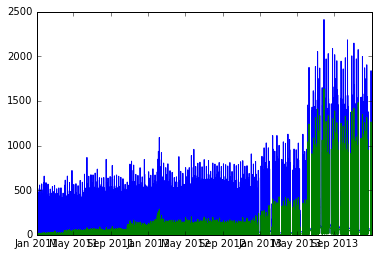
\includegraphics[scale=0.7]{img/telephonie_total.png}
\caption{Number of calls in the "Telephonie" category (green) and total number of calls (blue)}
\label{telephonie_total}
\end{figure}

We observe that the number of calls depends heavily on whether the day is a business day or not (see Figure~\ref{holiday}).

\section{Preprocessing}

In order to simplify the problem and after studying all the features, we decided to select only the date and the number of calls as base features.
So we need to preprocess the csv file to extract those. The preprocessing is done by our class \textbf{Preprocessor}. This step runs in two parts.
  \subsection{Get all the categorical features}
    We can classify the features of the dataset in two parts the numeric features and the categorical features. What we mean by categorical features


  \subsection{Create a valid dataset}
    After dataset exploration we quickly realised, that the data wasn't sorted at all which leads to the first step sorting all our data on the datetime (column number 1).
    This step has been done using Linux functionalities:
    \begin{lstlisting}[caption=Sort the csv file on the date, language=bash]
      head -1 train.csv > sortTrain.csv\;
      tail -n+2 train.csv | sort --parallel=8 -t ';' -k1 >> sortTrain.csv
    \end{lstlisting}

    When this step is done we want to create a numpy array of all the features which is quicker to load in order to train our model:

    \begin{algorithm}[H]
      \KwResult{Return X a numpy array of }
      x = 0\;
      \tcp{ We cannot load all the dataset on our machine we need to use chunk}
      \For{Each chunk (dataframe) of train.csv}{
        \If{not first chunk}{
          new\_df = concat tmp\_df with chunk\;
        }
        get the minimum date of new\_df\;
        get the maximum date of new\_df\;
        \tcp{We assume that for the maximum date we haven't all the information in this chunk}
        tmp\_df = all tuples which corresponds to the maximum date\;
        df = all the other tuples\;
        get the new maximum date of new\_df\;
        With the min and max dates create a list of all the time slot between the two dates\;
        \tcp{Preprocess the data}
        Group by \textbf{DATE} and \textbf{ASS\_ASSIGNMENT} on \textbf{CSPL\_RECEIVED\_CALLS} doing a sum\;
        Pivot all the value on \textbf{ASS\_ASSIGNMENT} to get at each time step the specific number of calls\;
        Complete the time step with unknown values with 0 and missing ASS\_ASSIGNMENT in the chunk\;
        x\_chunk = results of the previous operation \;
        x =  concatenation of x and x\_chunk \;
      }

      save x\;

     \caption{Preprocessing of the csv file (you can inspect the code in the method \_\_preprocess\_csv in preprocessing.py)}
    \end{algorithm}
